\documentclass{article}% [11pt]    % DRAFT at Arxiv
%   \documentclass[ journal]{IEEEtran}  % PUBLISH
% \documentclass[10pt,singlespace]{IEEEtran} % doublecolumn
% \documentclass[journal]{IEEEtran}
% \documentclass[draftcls,onecolumn]{IEEEtran}  % draftcls,
% \documentclass{sig-alternate}
% \documentclass{acm_proc_article-sp}

\usepackage{amsmath,amssymb,amsfonts,epsfig,amsfonts}
% \usepackage{amsthm} % used for \QED
\usepackage{cite}
\usepackage{graphicx}
%\usepackage{psfrag}
\usepackage{subfigure}
\usepackage{mathrsfs}
\usepackage{extarrows}  % For long equals
\usepackage{hyperref}
\usepackage{comment}  % for using \begin{comment}
\usepackage{pgfplots} % for using \addplot 
%\usepackage[colorlinks,
%            linkcolor=red,
%            anchorcolor=blue,
%            citecolor=green
%            ]{hyperref}    % For links to references
%\usepackage{amsthm}
\makeatletter

\baselineskip=40pt
\textheight 22.5truecm
\topmargin -0.5125truein
\textwidth 15.74truecm
\oddsidemargin -0.06truein
\evensidemargin -0.06truein
%\parindent=0pt
\parskip=0.1in
\renewcommand{\baselinestretch}{1.2}   %line space adjusted here

% On the Global Convergence of Block Coordinate Descent 
\title{ \bf Are local-mins Rare?
 \footnote{This is an informal note. }
} \vskip 1cm
\author{ Thomas Jefferson
}
\date{}
% \date{Nov, 2014}
% Example definitions.

\begin{document}
%\ninept
%
\maketitle
%

\begin{abstract}

Analyze nonconvex optimization from topology. 

\end{abstract}

\thispagestyle{empty}
%\newpage
%\tableofcontents
%\newpage
%\newpage

%%%%%%%%%%%%%%%%%%%%%%%%%%%%%%%%%%%%%%%%%%%%%%%%%%%%%%%%%%%%%%%%%%%%%%%%%%%%%
%%%%%%%%%%%----------------   section 1 Introduction --------%%%%%%%%%%%%%%%%
%%%%%%%%%%%%%%%%%%%%%%%%%%%%%%%%%%%%%%%%%%%%%%%%%%%%%%%%%%%%%%%%%%%%%%%%%%%%%



\section{Test Section}


\begin{comment}
This is an environment comment.
\end{comment}

\iffalse 
 This is commented by iffalse command, not comment.
 Not easy to be eliminated by this cleaning file. 
 \fi 

This is a percent \%.  Should stay here after running the cleaning file. 
% Whole line comment without newline

We add a figure for testing. 

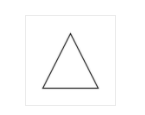
\includegraphics{images/im1_included.png}

If the code is correct, then the following figure should not appear in the cleaned tex file (
if the code is wrong in the sense that it only removes $\%$ but not the commands
after it, then the non-included figure would appear in the cleaned tex  file).
%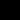
\includegraphics{images/im_not_included}

%This is a todo command\mytodo{Do this later}
% \mytodo{This is a todo command with a nested \textit{command}.

We can also check inputting other Latex Files.
This is a file in a sub-folder ``figures'', and we are supposed to see
one figure, but not two figures. 




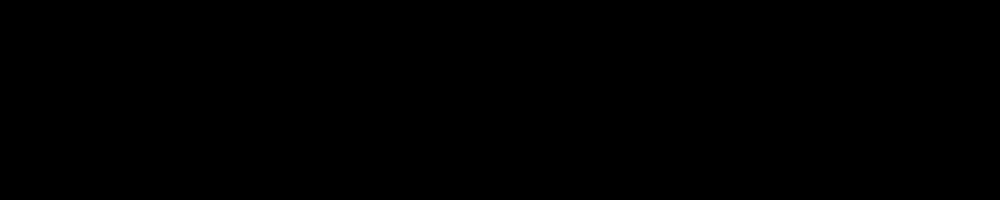
\includegraphics{images/im2_included.jpg}

% \addplot{figures/data_included.txt}

% \addplot{figures/data_not_included.txt}
\input{figures/figure_not_included_2.tex}




\section{Model}

This part is a test that the standard math formulas will not be affected after
running the cleaning file. 

Definition (LSC property): $\forall \bar{\alpha} \in G, \bar{x} \in L_f(\bar{\alpha}) \triangleq \{ x: f(x) \leq \bar{\alpha} \}$,
and $\forall$ sequence $\{ \alpha_i \} \rightarrow \bar{\alpha}$, we have 
$$
\exists x^i \in L_f(\alpha_i), \text{s.t. } \{ x^i\} \rightarrow \bar{x}. 
$$

Definition (GC property): For any two points $ f(\tilde{x}) < f(\bar{x}) $, there exists a sequence $ \{x^i\} \in C$ converging to $ \bar{x} $
such that 
\begin{equation}
f(x^i)\leq \frac{1}{i} f(\tilde{x}) + (1 - \frac{1}{i})f(\bar{x}). 
\end{equation} 


% \section{REFERENCES}
%  \bibliographystyle{IEEEbib}
 \vspace{0.3cm}
% \bibliography{refs}

{\footnotesize
\bibliography{refs}
}

%%--------------Bibliography------------------------------------------------------------------
%\begin{thebibliography} {TL99}
%\normalsize
%\bibitem{Candes1} E. J. Cand\`{e}s and B. Recht. Exact matrix completion via convex optimzation. Found. of Comput. Math.,
%
%
%%\bibitem{} J. Wright, A. Ganesh, S. Rao, and Y. Ma. Robust principal component analysis: Exact recovery
%% of corrupted low-rank matrices. arXiv:0905.0233, 2009.
%
%\end{thebibliography}

\end{document}



